\scanpage{11}
\mspage{3}
\diagram{\begin{tikzcd}[row sep=huge]
{\begin{gathered}\text{``Arbres plans'' \inserted{(non ponctuels)}}\\\text{(dans un plan pas néc. \deleted{orienté})}\end{gathered}}\arrow[d,leftrightarrow,"\simeq"]\\
{\begin{gathered}\text{polygones combinatoires, avec \deleted{involution} inv. sans}\\\text{pts fixes non pénétrante sur l'ens des}\\\text{\deleted{sommets}\inserted{arêtes.}}\end{gathered}}
\end{tikzcd}}
\par\noindent\rule{\linewidth}{.4pt}

Revenant au cas d'un graphe $\Gamma$ circularisé \inserted{général}, Topologiquement, le graphe top. $|\Gamma|$ se déduit de $|C|$ par \deleted{les identifications} un quotient par la relation d'équivalence suivante : on recolle l'arête $a$ et l'arête $\sigma_C^a$, en \uline{renversant} les \unsure{orientations} induites sur ces arêtes.

Dans le cas où $\Gamma$ est un arbre, on peut interpréter celui-ci \inserted{top${}^{t}$} en considérant $C$ comme le bord d'un disque orienté $D$, \unsure{subdivisé} en arêtes, et en joignant les ``centres'' des arêtes qui se correspondent par $\sigma_C$, de façon à ce que les segments obtenus ne se rencontrent pas.
\figure{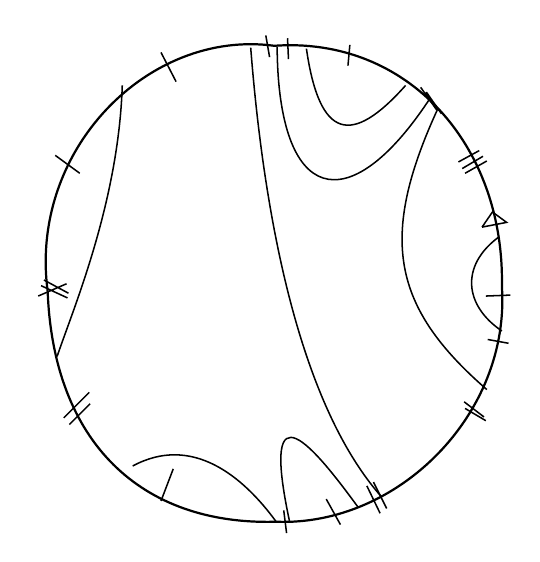
\begin{tikzpicture}[x=.012cm,y=-.012cm,line width=.55pt]
\draw[line width=.8pt] (95,1640).. controls (75,1490) and (202,1362)..(335,1380).. controls (476,1370) and (579,1485)..(576,1635).. controls (585,1770) and (466,1889)..(337,1884).. controls (194,1888) and (101,1800)..(95,1640);
\draw (174,1422).. controls (170,1547) and (121,1661)..(105,1709);
\draw (310,1382).. controls (326,1586) and (368,1766)..(448,1857);
\draw (338,1381).. controls (339,1547) and (413,1567)..(499,1437);
\draw (369,1383).. controls (383,1480) and (417,1486)..(474,1422);
\draw (508,1447).. controls (445,1584) and (460,1657)..(560,1744);
\draw (572,1583).. controls (532,1613) and (536,1655)..(576,1682);
\draw (185,1825).. controls (248,1791) and (302,1836)..(337,1884);
\draw (351,1883).. controls (319,1733) and (378,1806)..(424,1869);
\draw (215,1387)--(231,1418) (326,1369)--(330,1392) (349,1372)--(350,1394) (415,1379)--(413,1401);
\draw (490,1424)--(507,1448) (496,1429)--(512,1452);
\draw (530,1503)--(552,1491) (534,1510)--(556,1497) (537,1515)--(560,1502);
\draw (555,1572)--(581,1567)--(566,1556)--(555,1572);
\draw (559,1645)--(585,1644) (561,1691)--(583,1695);
\draw (536,1757)--(557,1773) (537,1764)--(559,1777);
\draw (433,1846)--(447,1875) (440,1842)--(454,1870);
\draw (390,1860)--(405,1887) (345,1872)--(348,1896) (228,1828)--(215,1862);
\draw (112,1774)--(139,1747) (118,1781)--(140,1759);
\draw (85,1645)--(115,1632) (88,1634)--(116,1647) (91,1628)--(117,1642);
\draw (103,1496)--(129,1515);
\end{tikzpicture}}
Les sommets de $\Gamma$ correspondent alors aux régions découpées dans $D$, et les arêtes orientées de $\Gamma$ aux frontières communes orientées,
\mspage{10}
